%!TEX TS-program = xelatex


%%%%%%%%%%%
% General %
%%%%%%%%%%%
\documentclass[A4,11pt]{article}
\NeedsTeXFormat{LaTeX2e}
\ProcessOptions\relax
\RequirePackage[left=1.5cm,top=1.5cm,right=1.5cm,bottom=1cm,nohead,nofoot]{geometry}


%%%%%%%%%%
% Colors %
%%%%%%%%%%
\RequirePackage{xcolor}
\definecolor{white}{RGB}{255,255,255}
\definecolor{darkgray}{HTML}{333333}
\definecolor{gray}{HTML}{4D4D4D}
\definecolor{lightgray}{HTML}{999999}
\definecolor{green}{HTML}{3F913F}
\definecolor{orange}{HTML}{FDA333}
\definecolor{purple}{HTML}{3C30B1}
\definecolor{red}{HTML}{FB4485}
\definecolor{pblue}{HTML}{0395DE}
\colorlet{fillheader}{white}
\colorlet{header}{gray}
\colorlet{textcolor}{gray}
\colorlet{headercolor}{gray}


%%%%%%%%%
% Fonts %
%%%%%%%%%
\RequirePackage[quiet]{fontspec}
\RequirePackage[math-style=TeX]{unicode-math}
\newfontfamily\bodyfont
[BoldFont=texgyreheros-bold.otf,
ItalicFont=texgyreheros-italic.otf,
BoldItalicFont=texgyreheros-bolditalic.otf]
{texgyreheros-regular.otf}
\newfontfamily\thinfont[]{Lato-Light.ttf}
\newfontfamily\headingfont[]{texgyreheros-bold.otf}
\defaultfontfeatures{Mapping=tex-text}
\setmainfont
[
  Mapping=tex-text, Color=textcolor,
  BoldFont=texgyreheros-bold.otf,
  ItalicFont=texgyreheros-italic.otf,
  BoldItalicFont=texgyreheros-bolditalic.otf
]
{texgyreheros-regular.otf}
\setmathfont{texgyreheros-regular.otf}


%%%%%%%%%%%%%
% Structure %
%%%%%%%%%%%%%
\RequirePackage{parskip}
\newcounter{colorCounter}
\def\@sectioncolor#1#2#3{%
  {%
    \color{%
      \ifcase\value{colorCounter}%
        pblue\or%
        pblue\or%
        pblue\or%
        pblue\or%
        pblue\else%
        pblue\fi%
    } #1#2#3%
  }%
  \stepcounter{colorCounter}%
}
\renewcommand{\section}[1]{
  \par\vspace{\parskip}
  {
    \LARGE\headingfont\color{headercolor}%
    \@sectioncolor #1%
  }
  \par\vspace{-1.2mm}
}
\renewcommand{\subsection}[2]{
  \par\vspace{.5\parskip}%
  \Large\headingfont\color{headercolor} #2%
  \par\vspace{.25\parskip}%
}
\pagestyle{empty}


%%%%%%%%%%%
% Section %
%%%%%%%%%%%
\setlength{\tabcolsep}{0pt}
\newenvironment{entrylist}{%
  \begin{tabular*}{\textwidth}{@{\extracolsep{\fill}}ll}
}{%
  \end{tabular*}
}
\renewcommand{\bfseries}{\headingfont\color{headercolor}}
\newcommand{\entry}[4]{
{
  \footnotesize #1}&\parbox[t]{16.0cm}{
    \textbf{#2} \\
    {\footnotesize\addfontfeature{Color=pblue} #3} \\
    {\footnotesize #4}\vspace{\parsep}
  } \\
}


%%%%%%%%%%%
% Imports %
%%%%%%%%%%%
\usepackage{afterpage}
\usepackage{hyperref}
\usepackage{color}
\usepackage{xcolor}
\usepackage{graphicx}
\RequirePackage{tikz}
\hypersetup {
    pdftitle={},
    pdfauthor={},
    pdfsubject={},
    pdfkeywords={},
    colorlinks=false,
    allbordercolors=white
}


%%%%%%%%%%%%
% Document %
%%%%%%%%%%%%
\begin{document}
\begin{minipage}[c]{0cm}
  \-\
\end{minipage}
\begin{minipage}[c]{0.2\textwidth}
  \begin{tikzpicture}
    \clip (0,0) circle (1.55cm);
    \node at (0.0, -0.7) {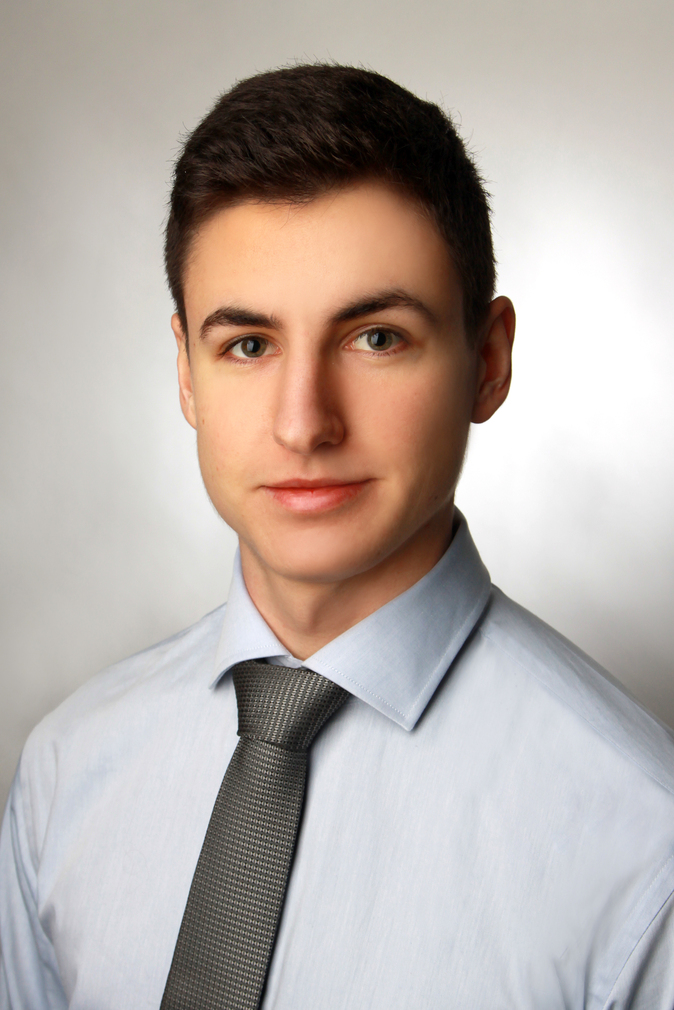
\includegraphics[width = 3.2cm]{diploma2}};    % (x, y) and width=zoom
  \end{tikzpicture}
  \hfill\vline\hfill
\end{minipage}
\begin{minipage}[c]{0.35\textwidth}
  {
    \fontsize{30pt}{62pt}\color{header}
    {\thinfont Tomasz}  {\bodyfont Kulik}
  }
  \textbf{phone:} +48 660 718 720 \\
  \href{mailto:}{\textbf{tomek.kulik2@}gmail.com} \\
  \href{https://linkedin.com/in/tomkulik}{\textbf{linkedin.com}/in/tomkulik} \\
  \href{https://github.com/kulikthebird}{\textbf{github.com}/kulikthebird} \\
\end{minipage}

\fcolorbox{white}{gray}{\parbox{\dimexpr\textwidth-2\fboxsep-2\fboxrule}{.....}}


\section{Experience}
\vspace{0.2cm}
\begin{entrylist}
  \entry
  {Jun/20 - }
  {Software Developer}
  {Luxoft, Wrocław, Poland}
  {
    I started work in a 5G project for a telco company. The work have been
    focused mainly on delivering new features to the services in the client's
    codebase. Working in the cloud environment became my standard way of thinking
    about software development.
    \begin{itemize}
      \setlength\itemsep{0.2em}
      \item Developing the 5G core software
      \item Implementing mainly new features
      \item Preparing a documentation and specification of new features
      \item Working on microservices in a cloud environment (\textbf{Azure})
      \item Testing new features
      \item Working with \textbf{Docker}, \textbf{Kubernetes}
      \item Programming: \textbf{Rust}, \textbf{Python3}, \textbf{C++}
    \end{itemize}
  }
  \entry
  {Aug/18 - Jun/20}
  {Engineer Software Developer}
  {Nokia, Wrocław, Poland}
  {
    After getting more experience in the project and programming skills I decided
    to focus more on the software development. Besides Python3, I started
    writing code for the telecommunication embedded system in C++14. I was
    also responsible for writing tests in TTCN-3 language. There were
    also other projects written mainly in Python in which I took part.
    \begin{itemize}
      \setlength\itemsep{0.2em}
      \item Developing \textbf{LTE} and \textbf{IoT} software in eNodeB component (Control Plane)
      \item Developing middleware for Radio Module (\textbf{init}, \textbf{systemd}, \textbf{Yocto})
      \item Implementing new features and maintaining legacy code
      \item Bug fixing, fault analysis
      \item Python3 and C/C++14 code reviewer
      \item Member of a \textbf{scrum team}
      \item Programming: \textbf{C++14}, \textbf{Python3}, \textbf{TTCN-3}, \textbf{VBA}, \textbf{Bash}
    \end{itemize}
  }
  \entry
  {Jun/15 - Aug/18}
  {Software Test Engineer}
  {Nokia, Wrocław, Poland}
  {
    I started work as a Working Student in Nokia by the end of a 2nd year of studies.
    I was part of a Q\&A team that worked on tests for base station. After few months I
    switched to the full time job and became a Test Engineer. To get a wider view of
    the project I took part in the review process as a code reviewer. The job gave
    me a chance of working close to the 'bear metal' and simultaneously to learn
    good practices in programming. 
    \begin{itemize}
      \setlength\itemsep{0.2em}
      \item Writing \textbf{automated tests}, preparing documentation of test plans
      \item Functional Testing, Integration Testing
      \item Working on a test environment for \textbf{LTE software} - U-plane and C-plane in eNodeB
      \item Python3 code review and co-author of ,,test guide''
      \item Member of a \textbf{scrum team}
      \item Programming: \textbf{Python3}, \textbf{RobotFramework}, \textbf{Bash}
    \end{itemize}
  }
\end{entrylist}

\newpage

\section{Education}
\vspace{0.1cm}
{\footnotesize
  My studies were focused mainly on a theory of Computer Science, though there were also practical exercises.
  I was using a number of programming languages during labs. I learned about algorithms used in various
  fields such as networking, distributed systems, coding and compression of data, compilers, data mining,
  optimization and so forth.
}

\begin{entrylist}
  \entry
  {2017 - 2019}
  {Master's Degree in Computer Science - Algorithmics}
  {Wrocław University of Science and Technology}
  {
    \emph{Faculty:} Fundamental Problems of Technology \\
    \emph{Thesis: ,,Filtering algorithms in constraints programming''.} \\
    \emph{Description and implementation of algorithms for domains reduction
      (constraints propagation) within IBM CPLEX environment. \textbf{C++11 / Optimization} }
  }
  \entry
  {2013 - 2017}
  {Bachelor's Degree in Computer Science}
  {Wrocław University of Science and Technology}
  {
    \emph{Faculty:} Fundamental Problems of Technology \\
    \emph{Thesis: ,,Computer modeling and solving geometry puzzles that require collision detection''.} \\
    \emph{Solver of 'Snake cube puzzle'. Application consists of an interactive 3D GUI that allows the user
      to manipulate the model and to solve it step by step. \textbf{C++11 / OpenGL} }
  }
\end{entrylist}


\section{Certifications}
\begin{itemize}
  \setlength\itemsep{-0.32em}
  \item {\small Best practices of object-oriented programming in C++ language}
  \item {\small ISTQB Certified Tester Foundation Level}
  \item {\small E-UTRAN/LTE Signalling}
  \item {\small LTE Cellular IoT}
\end{itemize}


\section{Tools}
\begin{itemize}
  \setlength\itemsep{-0.32em}
  \item \textbf{Cloud/DevOps:} Azure (basics), Docker, Jenkins, Kubernetes
  \item \textbf{Programming:} Bison, Cplex, GTest, OpenGL, PyTest, Yocto
  \item \textbf{Codebase and CI:} Fisheye, Gerrit, Git, Gitlab, Jenkins, Svn
  \item \textbf{Machine Learning:} Keras, Matplotlib, Numpy, Pandas, Scikit-learn
  \item \textbf{Operating Systems:} Linux, Windows
  \item \textbf{Misc:} Jira, Confluence, etc.
\end{itemize}


\section{Skills}
\begin{itemize}
  \setlength\itemsep{-0.32em}
  \item \textbf{Languages:} Polish (Native language), English (B2)
  \item \textbf{Programming:} C/C++ (experienced), Python (experienced), Rust (intermediate),
            Julia (intermediate), Go (basic), Prolog (basic), SQL (basic), VBA (basic)
  \item \textbf{Personal:} Team player, Fast learner, Sharing knowledge
\end{itemize}


\section{Interested in}
\begin{itemize}
  \setlength\itemsep{-0.32em}
  \item Dance and sport in general (trekking, snowboard, workout, etc.)
  \item Machine learning and algorithmics
  \item Guitar
\end{itemize}


{\tiny
  I hereby give consent for my personal data to be processed for the
  purpose of conducting recruitment for the position for which I am
  applying. I also consent to processing of my personal data
  for the purposes of any future recruitment processes.
}

\end{document}
